\documentclass[a4paper,11pt]{article}
\usepackage{lipsum}
\usepackage{xcolor}
\usepackage{hyperref}
\usepackage{multicol}
\usepackage{abstract}
\usepackage{caption}
\usepackage{fontspec}
\usepackage{tabto}
\usepackage{ragged2e}
\usepackage{indentfirst}
\setmainfont{Times New Roman}
\renewcommand{\abstractname}{Summary}
\renewcommand{\figurename}{Fig.}
\renewcommand{\tablename}{Tab.}
\renewcommand{\contentsname}{Table of Contents}
\renewcommand{\refname}{Bibliography}
\renewcommand{\baselinestretch}{1.2}
\setcounter{secnumdepth}{2}
\setcounter{tocdepth}{2}

\begin{document}
\title{Field Notes}
\author{Anonymous}
\maketitle
\thispagestyle{empty}

\begin{abstract}
\lipsum[1][1-3]
\end{abstract}

\section{Two columns}
\begin{multicols}{2}
\lipsum[2]
\columnbreak
\lipsum[3]
\end{multicols}

\section{Text features}
\begin{justify}
Justified text with \textbf{bold}, \textit{italic}, \textsl{slanted}, \textsc{Small Caps}, \texttt{mono}, \textsf{sans},
\textup{upright}, \emph{emphasis with \emph{nested} emphasis}, \textbf{\textit{bold italic}},
\textsuperscript{sup} and \textsubscript{sub}.
\end{justify}
\begin{Center}
Centered with ragged2e.
\end{Center}
\begin{FlushRight}
Flush right with ragged2e.
\end{FlushRight}

Sizes: {\tiny tiny} {\scriptsize script} {\footnotesize foot} {\small small} {\normalsize normal} {\large large} {\Large Large} {\LARGE LARGE} {\huge huge} {\Huge Huge}.

Special characters: \& \% \$ \# \_ \{ \} \textbackslash{} \textasciitilde{} \textasciicircum{} \textless{} \textgreater{} \textbar{} \slash{} \textperiodcentered{} \textbullet{} \dag{} \ddag{} \textdagger{} \textsection{} \textquotedbl{} \guillemotleft{}a\guillemotright{} \textendash{} \textemdash{} \textellipsis{}.

Accents: \'e \`a \^o \"u \~n \c{c} \v{s} \u{a} \H{o} \r{a} \k{a} \={o} \.{z} \aa{} \AA{} \ae{} \oe{} \ss{} \o{} \l{} \i{} \j{}.

Logos: \LaTeX{}, \TeX{}, \LaTeXe{}, \BibTeX{}, \XeLaTeX{}.

Spaces: a\,b a\:b a\;b a\!b a\quad b a\qquad b a~b a\enspace b a\thinspace b a\ b.

Links: \href{https://example.com}{a link}, \url{https://example.com}, \hyperref[sec:end]{a section link}, \hyperlink{target}{jump} and \hypertarget{target}{here}.

\begin{figure}[htb]
\centering
\captionsetup{width=0.8\textwidth}
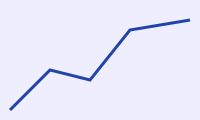
\includegraphics[width=.5\linewidth]{plot.svg}
\caption{A plot.}\label{fig:a}
\end{figure}

\section{End}\label{sec:end}
\lipsum[4-5]
\begin{center}
\rule{0.5\textwidth}{1pt}
\end{center}
\end{document}
